\chapter{Continental}
	\section{Organisation de l'entreprise}
		\subsection{Continental AG}
		Continental AG est une entreprise allemande dont le siège principal est à Hanovre. Il s’agit d’une Société Anonyme dont le président du comité de direction est depuis le 11 septembre 2001 Manfred Wennemer. Plus de 170.000 collaborateurs qui sont employés dans plus de 200 sites dans 45 pays appartenant à l'entreprise. En Allemagne Continental est une S.A. numéro un du marché de Production de pneu toutefois il s’agit aussi d’un équipementier automobile important. 

		Continental AG a été fondée en 1871 et est à nouveau membre depuis août 2003 de DAX. En 2007 elle a obtenu un chiffre d'affaires 16 milliards d'Euros. L'entreprise est composée de 2 grands groupes auxquels sont rattachées 5 branches (Tires est composé de branches voir Figure 2).

		\subsection{Histoire de l'entreprise}
		Continental est fondée en 1871 comme société anonyme sous le nom de <<Continental-Caoutchouc- und Gutta-Percha Compagnie>> par neuf banquiers et industriels de Hanovre (Allemagne).

		Continental dépose l'emblème du cheval comme marque de fabrique à l'Office impérial des brevets de Hanovre en octobre 1882. Il est aujourd'hui encore protégé en tant que marque distinctive.

		Le fabricant de pneus allemand débute son expansion à l'international en tant que sous-traitant automobile international en 1979, expansion qu'il n'a cessé de poursuivre depuis de manière systématique.
		
		Entre 1979 et 1985 Continental pose définitivement un pied en Europe avec le rachat l'acquisition des activités pneumatiques européennes de l'américain Uniroyal Inc. Et de la marque de pneus autrichienne Semperit.

		En 1995 est créée la Division Automotive Systems pour intensifier les activités <<systèmes>> avec l'industrie automobile.

		Pour renforcer sa position sur les marchés américain et asiatique, Continental fait l'acquisition en 2001 du spécialiste international de l'électronique Temic, qui dispose de sites de production en Amérique et en Asie. Deux autres reprises ont lieu en 2001. Continental reprend la majorité des parts de deux entreprises japonaises produisant des composants d'actionnement des freins et des freins à disques.

		En 2004, le plus grand spécialiste mondial de la technologie du caoutchouc et des plastiques naît de la fusion entre Phoenix AG et ContiTech.

		En juillet 2007 Continental réalise son plus gros rachat sur le fournisseur automobile Siemens VDO Automotive

		\begin{figure}[H]
			\centering
			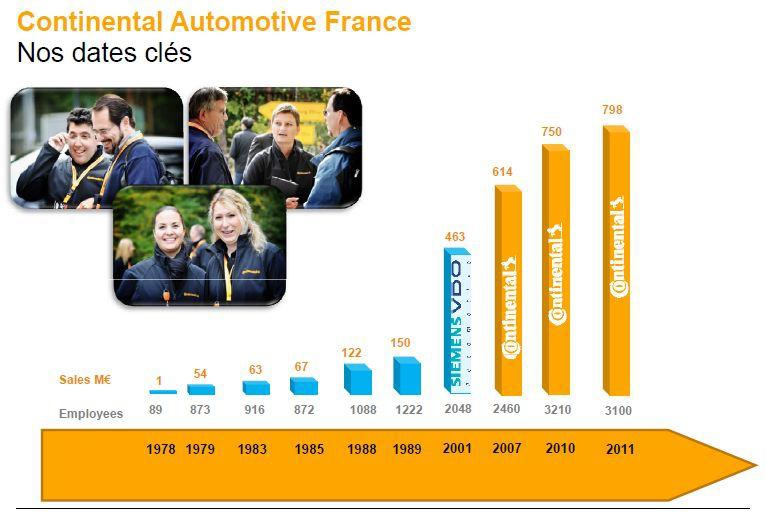
\includegraphics[width=10cm]{contents/images/datesCles.jpg}
			\caption{Dates clés}
			\label{fig:datesCles}
		\end{figure}
		\subsection{Activités des différentes braches}
	\section{Le contexte de l'équipe Vérification \& Validation}
		\subsection{L'équipe}
		\subsection{Le besoin}
